\newpage
\section{All You Need Are Reflections}

In this activity, we are going to explore how reflections are related
to rotations. When doing this activity, you don't need to worry about
the actual matrices involved. 

\begin{prob}
You may have noticed that $180^\circ$ rotations and horizontal (or
vertical) reflections seem kind of similar. Explain how they are
similar, then explain how they are different.
\end{prob}


\begin{prob}
Explain how to express a $180^\circ$ as the composition of two
reflections. Work out some examples to give evidence that you are
correct.
\end{prob}
Consider the following ``F'' shape:
\[
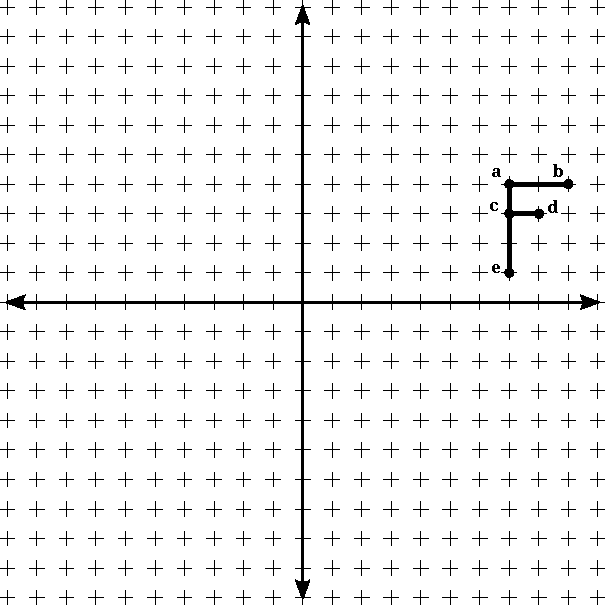
\includegraphics{../graphics/planeR.pdf}
\]
\begin{prob}
Reflect our shape across the line $y=x$. Label the reflection of the
points with a prime---the reflection of $\mathbf{a}$ across $y=x$ is
$\mathbf{a}'$.
\end{prob}

\begin{prob}
Reflect our new shape across $x=0$. Label the reflection of the points
with another prime---the reflection of $\mathbf{a}'$ across $x=0$ is
$\mathbf{a}''$.
\end{prob}

\begin{prob}
Through how many degrees was our original shape rotated about the
origin?
\end{prob}


\begin{prob}
Letting $\mathbf{o}$ be the origin and ``$-$'' be a place-holder, use
a protractor to fill in the described angles:
\[
{\renewcommand{\arraystretch}{2}
\begin{tabular}{|c|c|c|c|}\hline
$-$ & $-$, $\mathbf{o}$, and $-'$ & $-'$, $\mathbf{o}$, and $-''$ & $-$, $\mathbf{o}$, and $-''$ \\ \hline\hline
$\mathbf{a}$ & & & \\ \hline 
$\mathbf{b}$ & & & \\ \hline 
$\mathbf{c}$ & & & \\ \hline  
$\mathbf{d}$ & & & \\ \hline  
$\mathbf{e}$ & & & \\ \hline        
\end{tabular}}
\]
What do you notice?
\end{prob}



\begin{prob}
Letting $\mathbf{o}$ be the origin and ``$-$'' be a place-holder, use
a protractor to fill in the described angles:
\[
{\renewcommand{\arraystretch}{2}
\begin{tabular}{|c|c|c|c|}\hline
$-$ & $-$, $\mathbf{o}$, and $y=x$ &  $-'$, $\mathbf{o}$, and $x=0$ & \text{the sum} \\ \hline\hline
$\mathbf{a}$ & & & \\ \hline 
$\mathbf{b}$ & & & \\ \hline 
$\mathbf{c}$ & & & \\ \hline  
$\mathbf{d}$ & & & \\ \hline  
$\mathbf{e}$ & & & \\ \hline        
\end{tabular}}
\]
What do you notice?
\end{prob}


\begin{prob}
Suppose I want to rotate an object $\theta^\circ$ around the origin
using two reflections. Can you conjecture how the lines should be
placed on the plane? Draw pictures to help with your explanation.
\end{prob}

